\section{\label{sec:experiment}Experiments}
%\gn{You need at least one sentence of lead-in here.}
In this section, we first discuss the experimental results of DDS on image classification, an instance of the general classification problem using Algorithm \ref{alg:image_classification_dds}. Then we demonstrate the effectiveness of DDS on a special case of multilingual NMT using Algorithm \ref{alg:nmt_dds}.

\subsection{\label{exp:image_classification}Image Classification}

\paragraph{Settings.} We apply our method on two established image classification datasets, CIFAR-10~\citep{cifar10} and ImageNet~\citep{imagenet}. For each dataset, we consider two settings: a reduced setting where only roughly 10\% of the training labels are used, and a full setting, where all labels are used. Specifically, the reduced setting for CIFAR-10 uses the first $4000$ examples in the training set, and with ImageNet, the reduced setting uses the first $102$ TFRecord shards as pre-processed by~\citet{imagenet_generalize_better}. We use the size of $224 \times 224$ for ImageNet.

\paragraph{Models and Baselines.} For CIFAR-10, we use the pre-activation WideResNet-28~\citep{wide_res_net}, with a width factor $k=2$ for the reduced setting and $k=10$ for the normal setting. For ImageNet, we use the post-activation ResNet-50~\citep{res_net}. Our baselines are the standard implementations of these models, where we reproduce the numbers commonly reported in the literature~\citep{wide_res_net,res_net,resnext}.

\paragraph{Training details.} The batch sizes for CIFAR-10 and for ImageNet are $128$ and $4096$, running for 200K steps and 40K steps, respectively. We use the cosine learning rate decay schedule~\citep{cosine_lr}, starting at $0.1$ for CIFAR-10 and $3.2$ for ImageNet, both with $2000$ warmup steps. We use the standard Momentum update for the model parameter $\theta$, and the derived Momentum update rule in Section~\ref{sec:grad_of_optimizers} for the distribution parameter $\psi$, both with the momentum rate of $0.9$. We maintain a moving average of all model parameters with the rate of $0.999$. Following~\citet{imagenet_generalize_better}, we treat the moving statistics of batch normalization~\citep{batch_norm} as \textit{untrained parameters} and also add them to the moving averages.

Our experiments are conducted on the second generation of Tensor Processing Units (TPUv2). We discuss three important implementation details to improve the training efficiency of ImageNet models. First, each batch of $4096$ training instances for ImageNet is processed in parallel on $32$ TPU cores, each working on $128$ images. When we compute $p(\hat{x}, \hat{y}; \psi)$ (\cf~Section \ref{sec:image_method}), the softmax function is computed \textit{locally on each core} to reduce the synchronization overhead. Second, since we do not need the parameters $\psi$ of the distribution model, we ignore all batch normalization moving average updates when we pass images through $p(\hat{x}, \hat{y}; \psi)$. We also only batch-normalize the distribution model locally on each TPU core. Controlled profiling measures show that the aforementioned details speed up the training process by almost $2.5 \times$. Third, following~\citet{neural_combi} and~\citet{enas}, for ImageNet, we apply a $\tanh$ activation to the logits prior to the softmax to compute $p(\hat{x}, \hat{y}; \psi)$, to soften the softmax distribution and prevents the $p(\hat{x}, \hat{y}; \psi)$ to collapse into always choosing a particular example. We note that all these three tricks are not needed for our experiments on CIFAR-10, where the batch size is much smaller.

%\begin{wraptable}{l}{0.7\textwidth}
\begin{center}
  \begin{tabular}{llll}
    \multicolumn{4}{c}{\textbf{CIFAR-10} ($\text{mean} \pm \text{std}$ over $10$ runs)} \\
  \toprule
    \textbf{Portion} &
    \textbf{Model} &
    \textbf{Baseline} &
    \textbf{\dds}
    \\
  \midrule
    4K &
    WideResNet-28-2 &
    $82.60 \pm 0.17$ & % 6109331
    $\mathbf{83.63 \pm 0.29}$ % 6109486
    \\
    Full &
    WideResNet-28-10 &
    $95.55 \pm 0.15$ &  % 6153155
    $\mathbf{96.31 \pm 0.13}$  % 6170380
    \\
  \bottomrule
    \\
    \multicolumn{4}{c}{\textbf{ImageNet} ($\text{Top-1}/\text{Top-5}$)} \\
    \toprule
    \textbf{Portion} &
    \textbf{Model} &
    \textbf{Baseline} &
    \textbf{\dds}
    \\
  \midrule
    10\%  & ResNet-50 &
    $56.36 / 79.45$ & % 5267621/workUnits/118
    $\mathbf{56.81 / 79.51}$   % 6020481/workUnits/18
    \\  
    Full & ResNet-50 &
    $76.51 / 93.20$ & % https://arxiv.org/abs/1810.12890
    $\mathbf{77.23 / 93.57}$ % 6800564/workUnits/39
    \\
    \bottomrule
  \end{tabular}
  \captionof{table}{\label{tab:image_classification_results}Image classification accuracy. Higher is better.}
\end{center}
%\end{wraptable}

\paragraph{Results.} Results are presented in Table~\ref{tab:image_classification_results}. As can be seen, \dds~improves the performance of all tasks considered. In our intuitions, \dds~provides an extra degree of freedom to train the models, namely the per-example scaling of gradients. This extra degree of freedom is well-utilized by the $p(\hat{x}, \hat{y}; \psi)$ distribution, leading to the improvements.


\subsection{Multilingual NMT}
\paragraph{Dataset.}
We use the 58-language-to-English TED dataset~\citep{ted_pretrain_emb}. 
Following setups in prior work~\citep{ted_pretrain_emb,rapid_adapt_nmt,SDE}, we use three low-resource languages~(LRL) Azerbaijani~(aze), Belarusian~(bel), Galician~(glg) to English,
and a slightly higher-resource dataset, Slovak~(slk) to English. Each language is paired with its most related high-resource language~(HRL), namely Turkish~(tur), Russian~(rus), Portugese~(por), and Czech~(ces) respectively, with the statistics of the datasets listed in Appendix~\ref{app:nmt_data}. Our goal is to optimize the usage of the data from the 8 languages for training NMT models for each LRL. 

\paragraph{Baselines.} We compare our method against three strong baselines: 1) All: all 8 languages are used for training without any data selection; 2) Bi: we train on the combined datasets of each LRL and its related HRL, which is a special case of data selection that requires prior linguistic knowledge; 3) TCS~\citep{TCS}: the state-of-the-art data selection method for multilingual NMT. Given a target sentence, TCS conditionally samples a source sentence from the candidate languages based on simple heuristics such as vocabulary overlap.

\paragraph{Implementation.} Here we clarify several design choices for Algorithm \ref{alg:nmt_dds}. To model the distribution $p(S_i|y;\psi)$, we use a 2-layer feed-forward network with hidden size of 32. The input vector for the network is a vector of size of source languages $n$, representing which of the languages contain a corresponding source sentence for a given target sentence $y$. We use the standard Adam update rule with learning rate of 0.001 for the NMT model parameter $\theta$, and the derived Adam update rule from Section~\ref{sec:grad_of_optimizers} with learning rate~0.0001 for the distribution parameter $\psi$. 

We test two different settings for using DDS for multilingual  NMT: 1) TCS+DDS: we pretrain the network with the heuristic distribution from TCS before the DDS training process
%. K in Algorithm \ref{alg:nmt_dds} is set to be 50,000; 
2) Uniform+DDS: we train the network for $\psi$ from scratch. %At the start of training, K is set to be 5,000 to encourage exploration; after updating $\psi$ for 5 times, we also set it to 50,000.
We run all experiments with 3 different random seeds and pick the median for each method. Additional hyperparameters are listed in Appendix~\ref{app:nmt_hparam}.

\paragraph{Results.}
\begin{wraptable}{l}{0.6\textwidth}
\begin{center}
    \begin{tabular}{l|cccc}
    \toprule
    \textbf{Model} & \textbf{aze} & \textbf{bel} & \textbf{glg} & \textbf{slk} \\
    \midrule
    All & 10.31 & 17.21 & 26.05 & 27.44 \\
    Bi & 10.34 & 15.31 & 27.41 & 25.92 \\
    TCS & 11.18 & 16.97 & 27.28 & 27.72 \\
    \midrule
    TCS+DDS & \textbf{11.84} & \textbf{17.74} & \textbf{27.78} & 27.74 \\
    %Uniform & 9.54 & 14.75 & 25.11 & 26.30 \\
    Uniform+DDS & 10.74 & 17.24 & 27.32 & \textbf{28.20} \\
    \bottomrule
    \end{tabular}
     \captionof{table}{\label{tab:nmt_result}BLEU score. Higher is better.}
\end{center}
\end{wraptable}
The results of the baselines and our method are listed in Table \ref{tab:nmt_result}. In our setting, training on all 8 languages (All) performs better than using a single related language (Bi) on~2 of the~4 languages, probably because the number of languages in the training corpus is not very large. However, the All method requires significantly more training steps than the other methods, and has found to be worse than Bi when the number of training languages is large~\citep{rapid_adapt_nmt,TCS}. The heuristic-based data selection method (TCS) effectively improves over or performs comparably with the Bi baseline. In general, DDS outperforms all strong baselines on all 4 languages. When the data selection distribution is initialized with the heuristics from TCS, it consistently improves over TCS on all 4 languages~(TCS+DDS). Even without heuristic initialization, TCS+Uniform still achieves competivitve performance compared to the baselines. Notably, for slk, the best performing method is discovered by DDS without heuristic initialization.

\begin{center}
  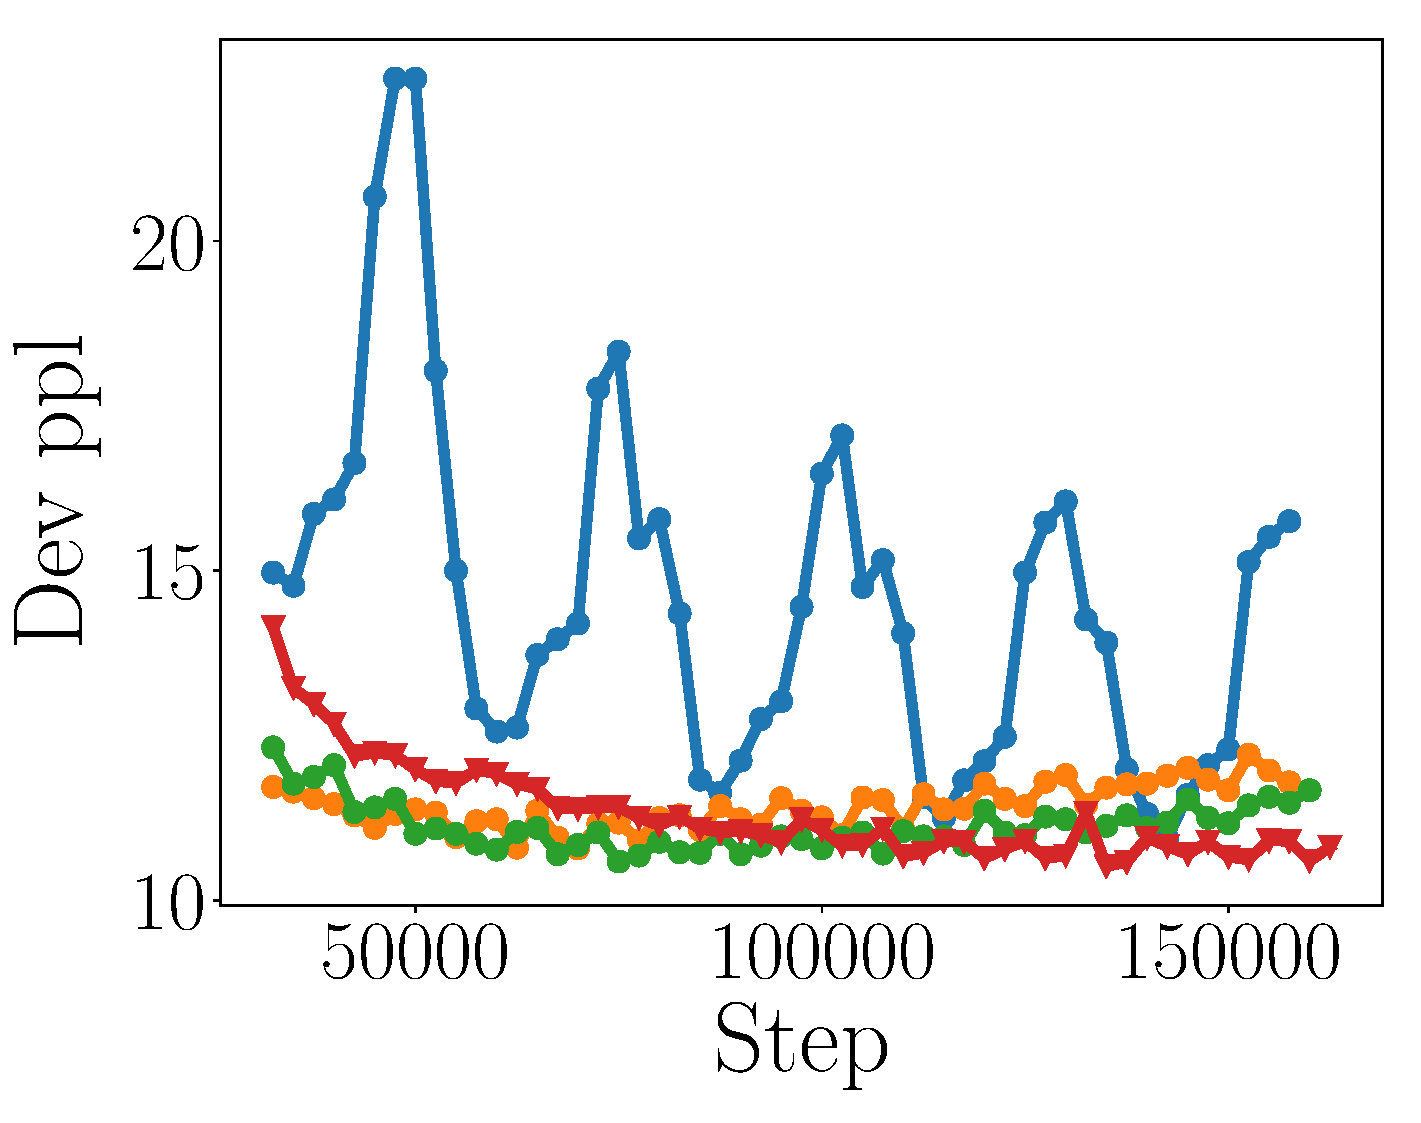
\includegraphics[width=0.245\columnwidth]{figs/aze_devppl_plot.eps}
  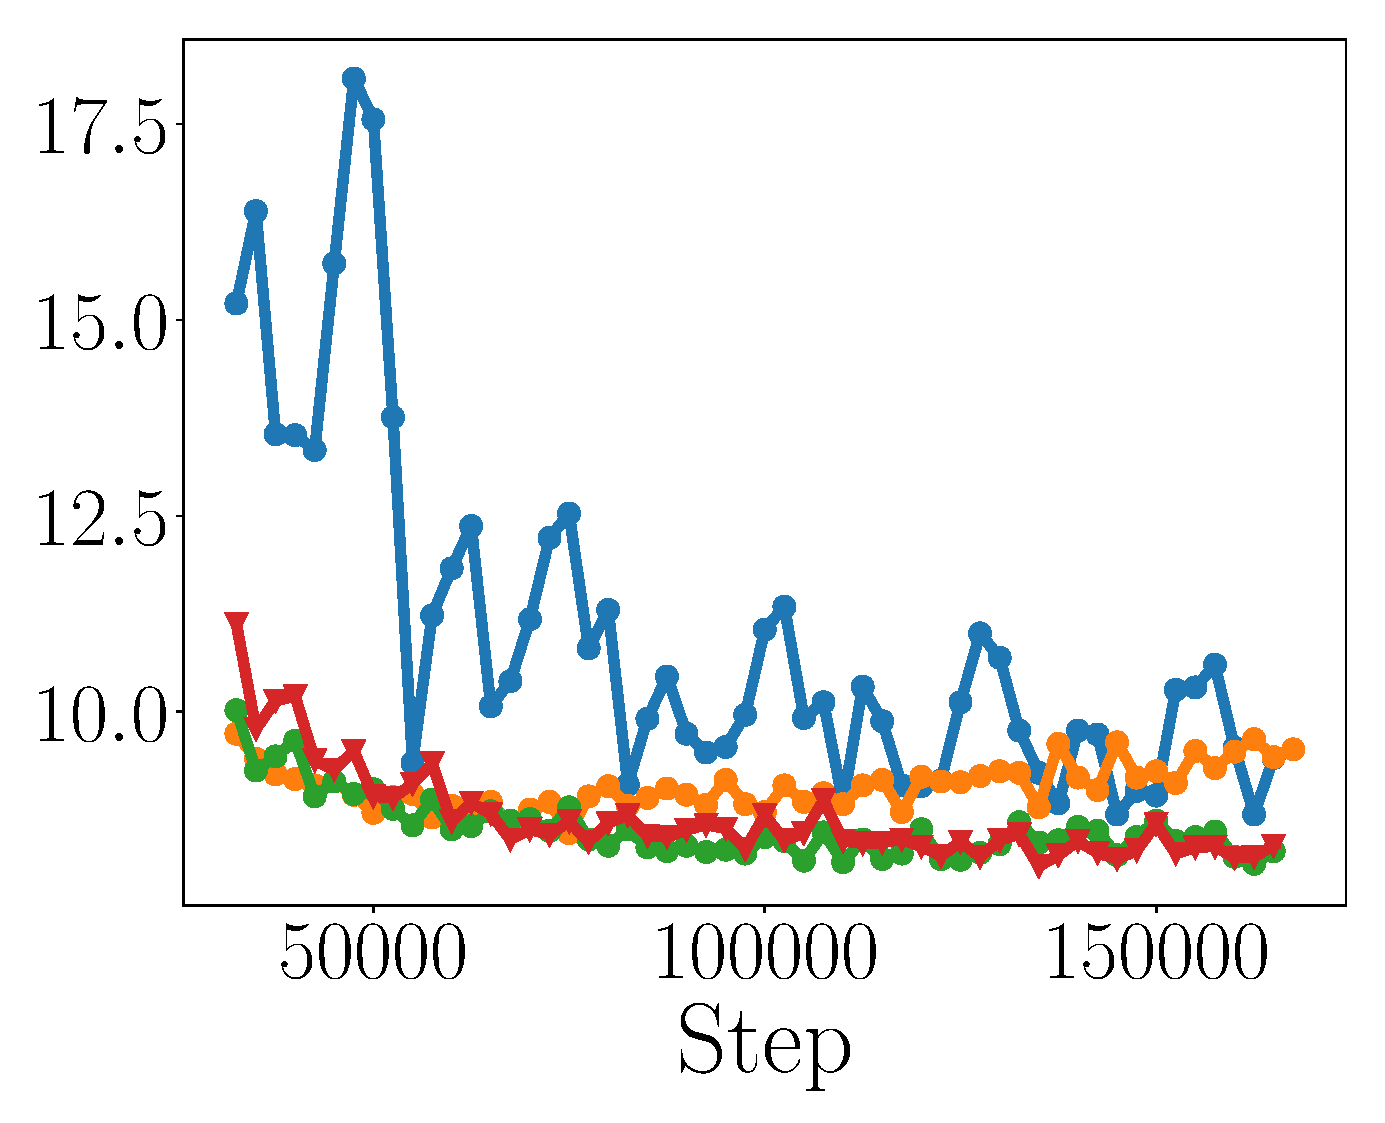
\includegraphics[width=0.23\columnwidth]{figs/bel_devppl_plot.eps}
  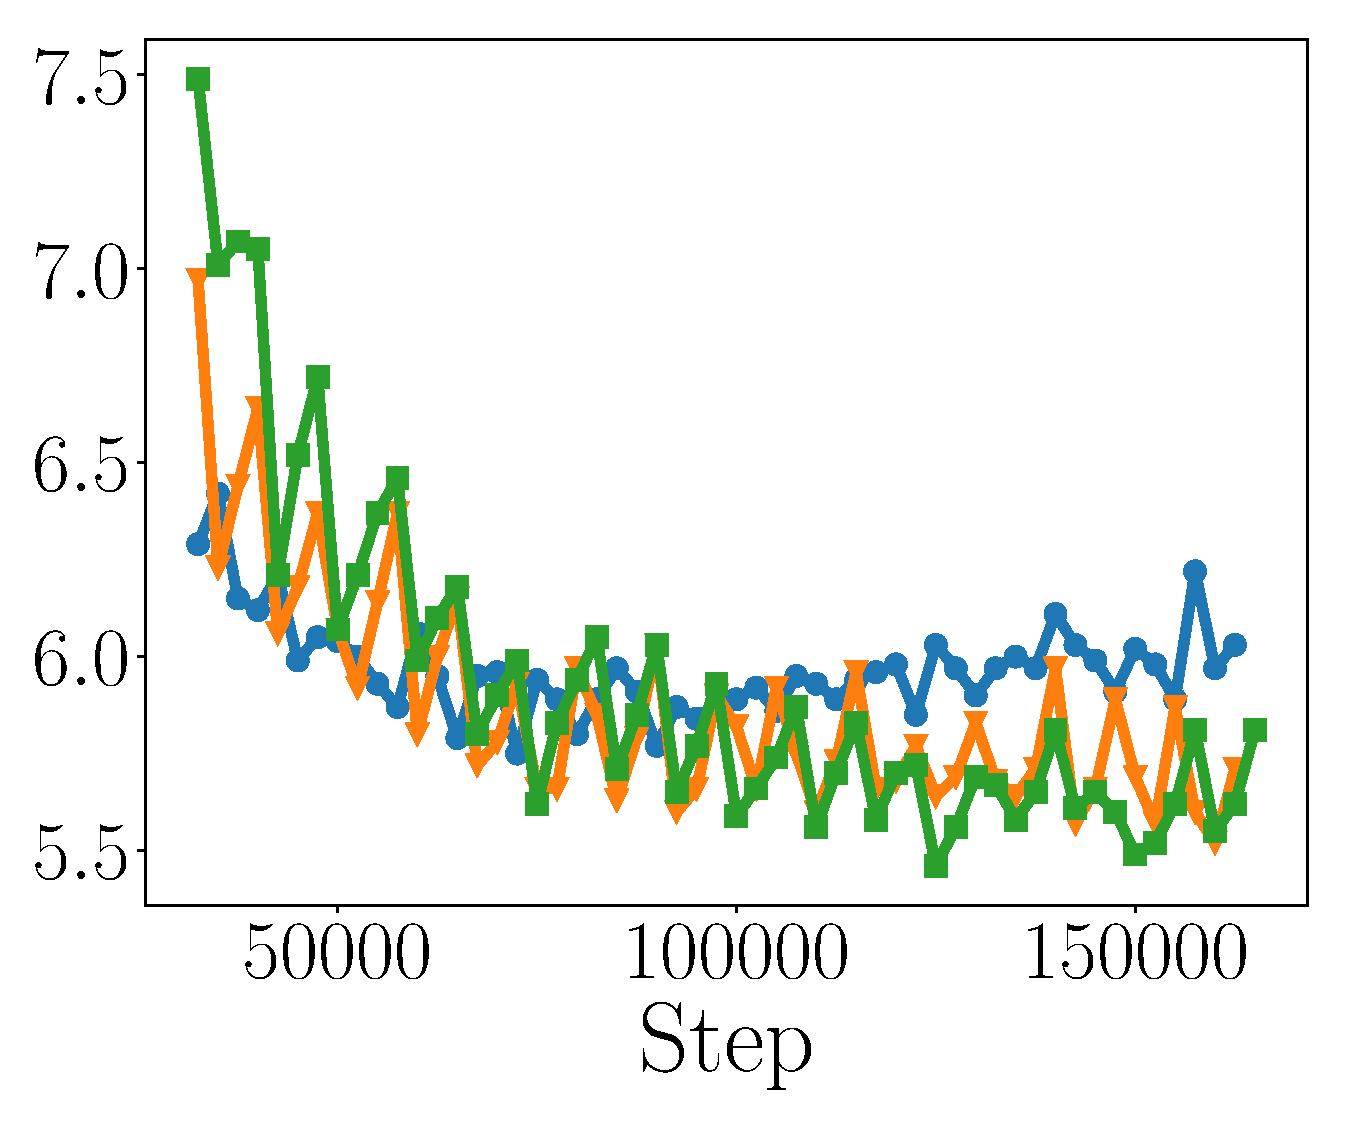
\includegraphics[width=0.23\columnwidth]{figs/glg_devppl_plot.eps}
  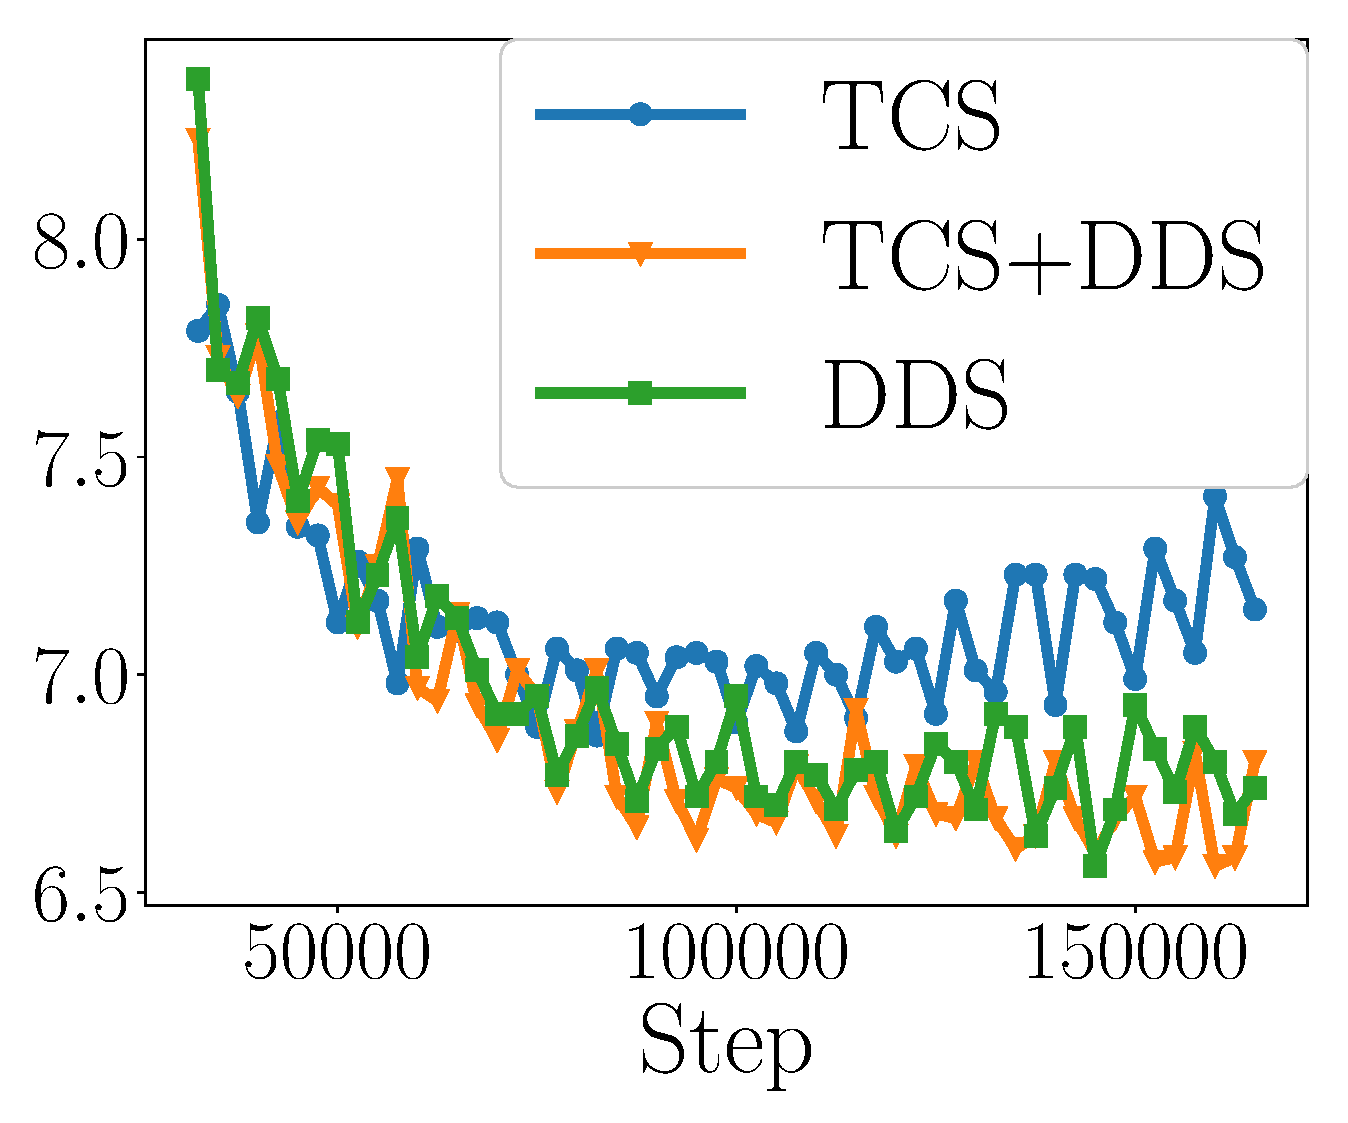
\includegraphics[width=0.23\columnwidth]{figs/slk_devppl_plot.eps}
  \captionof{figure}{\label{fig:nmt_converge}Development set perplexity vs. training steps. \textit{From left to right}: aze, bel, glg, slk.}
\end{center}
\paragraph{Training curve.} We plot the dev set perplexity over the course of training in Figure \ref{fig:nmt_converge}. DDS, with or without initialization with the heuristic distribution from TCS, allows the model to reach lower dev perplexity than TCS for all 4 languages.

\begin{center}
  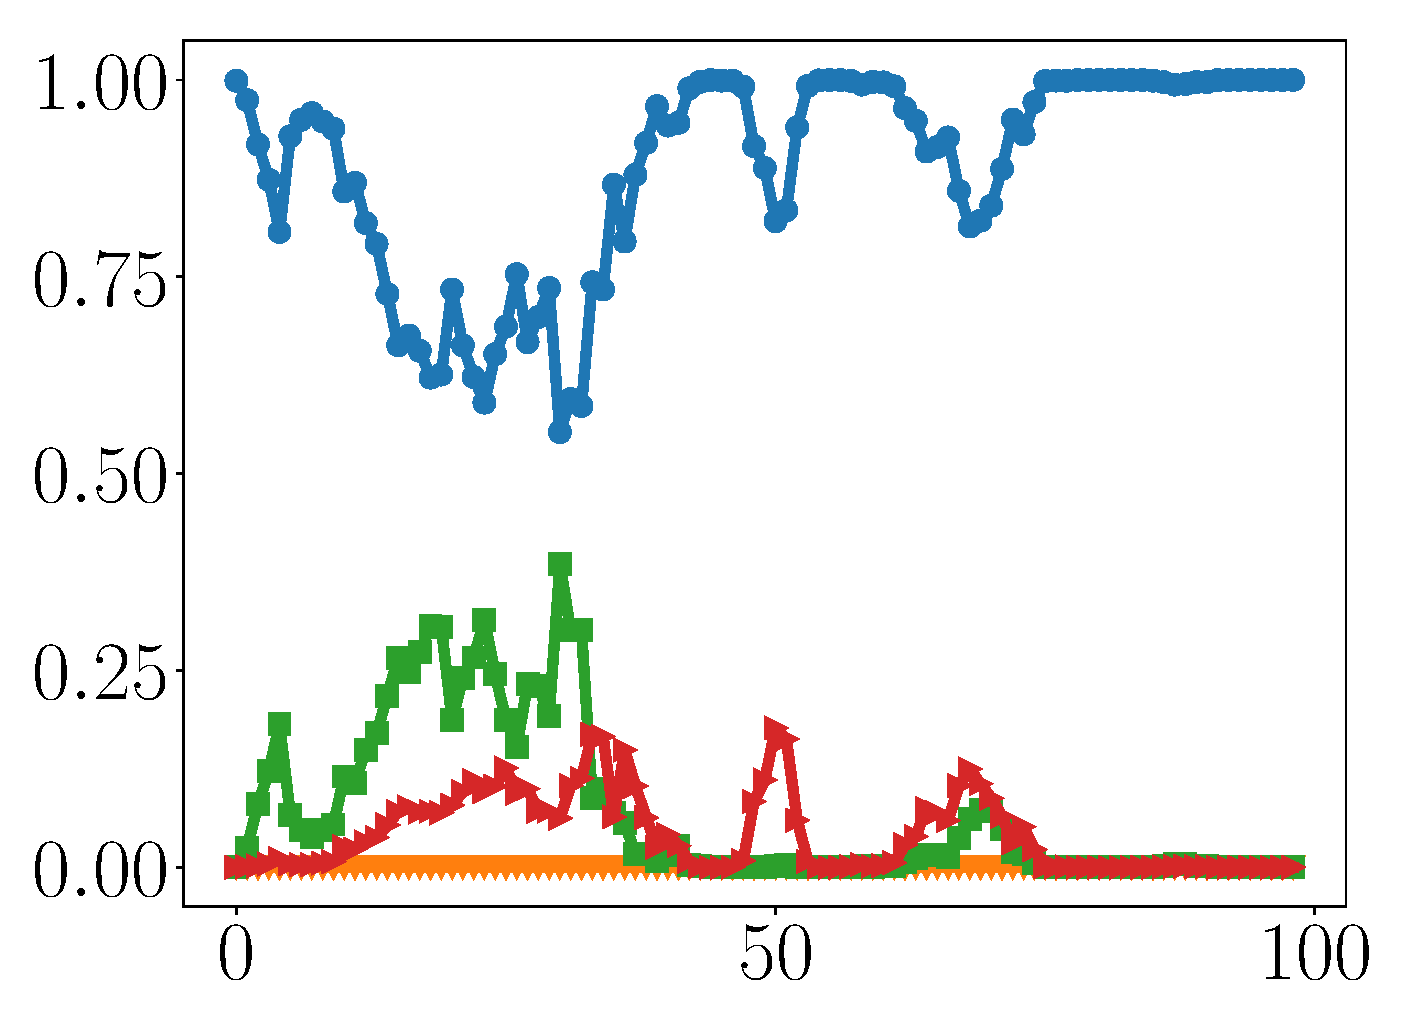
\includegraphics[width=0.22\columnwidth]{figs/aze_hs_probs_plot.eps}
  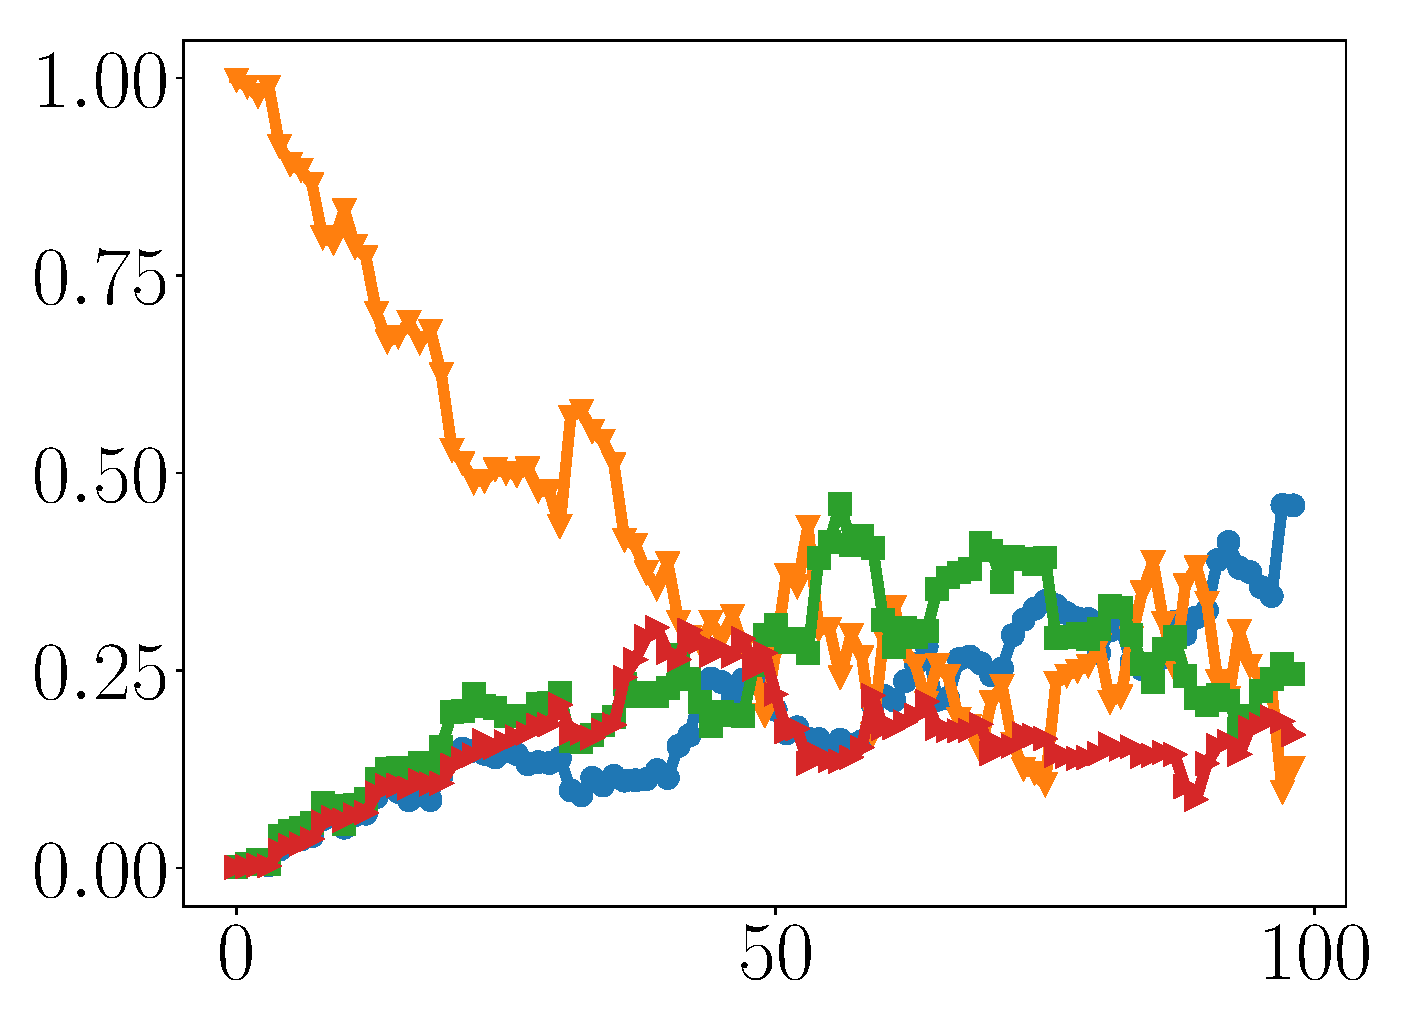
\includegraphics[width=0.22\columnwidth]{figs/bel_hs_probs_plot.eps}
  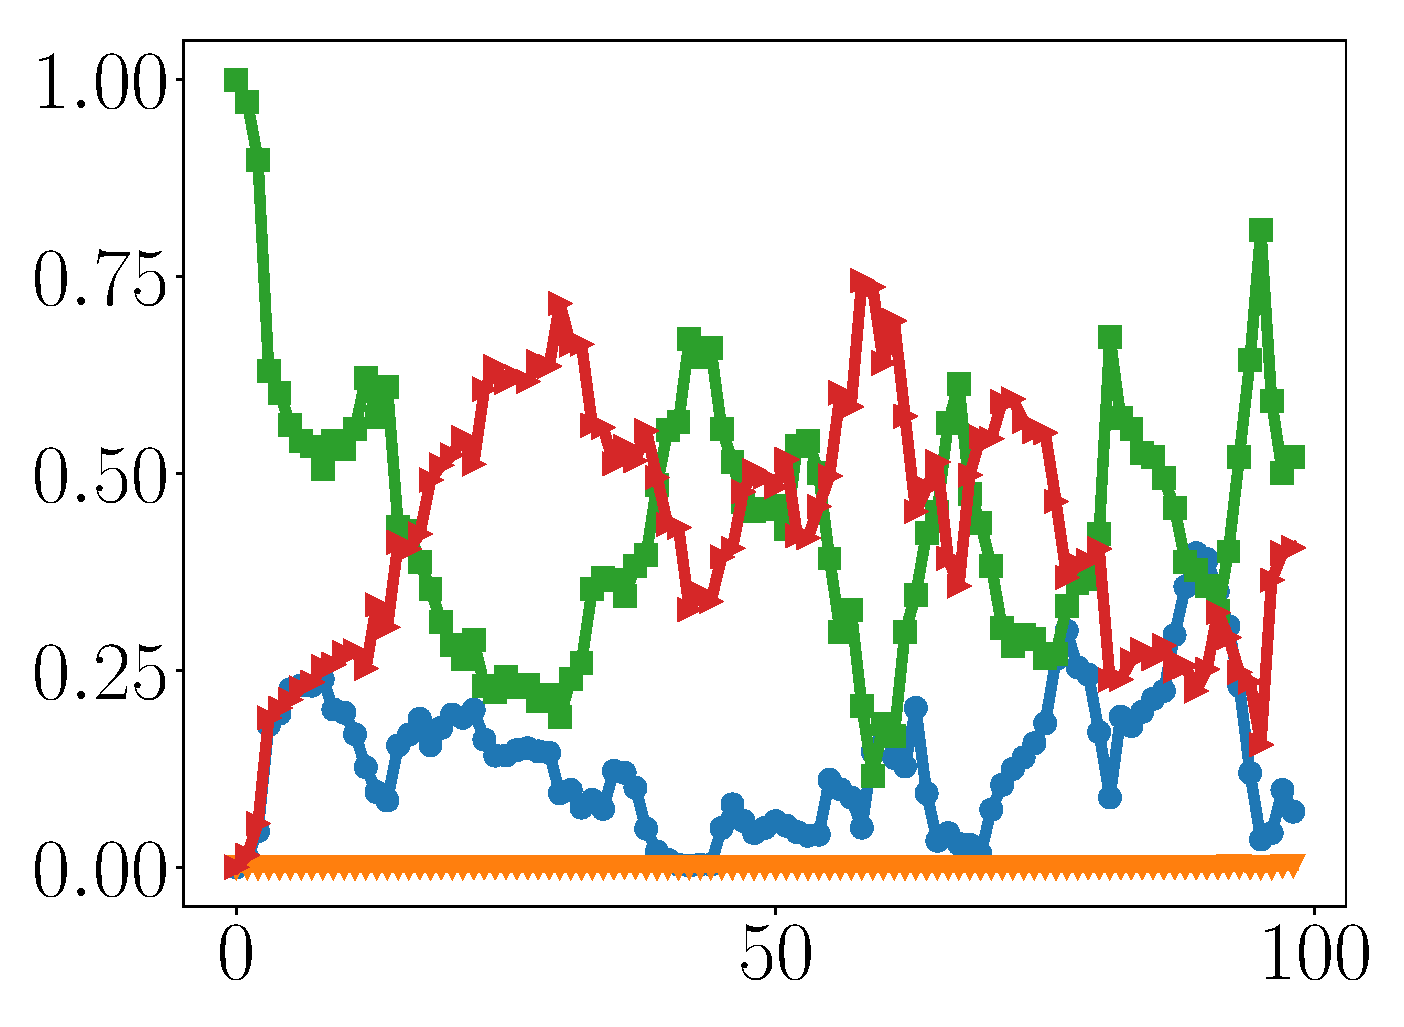
\includegraphics[width=0.22\columnwidth]{figs/glg_hs_probs_plot.eps}
  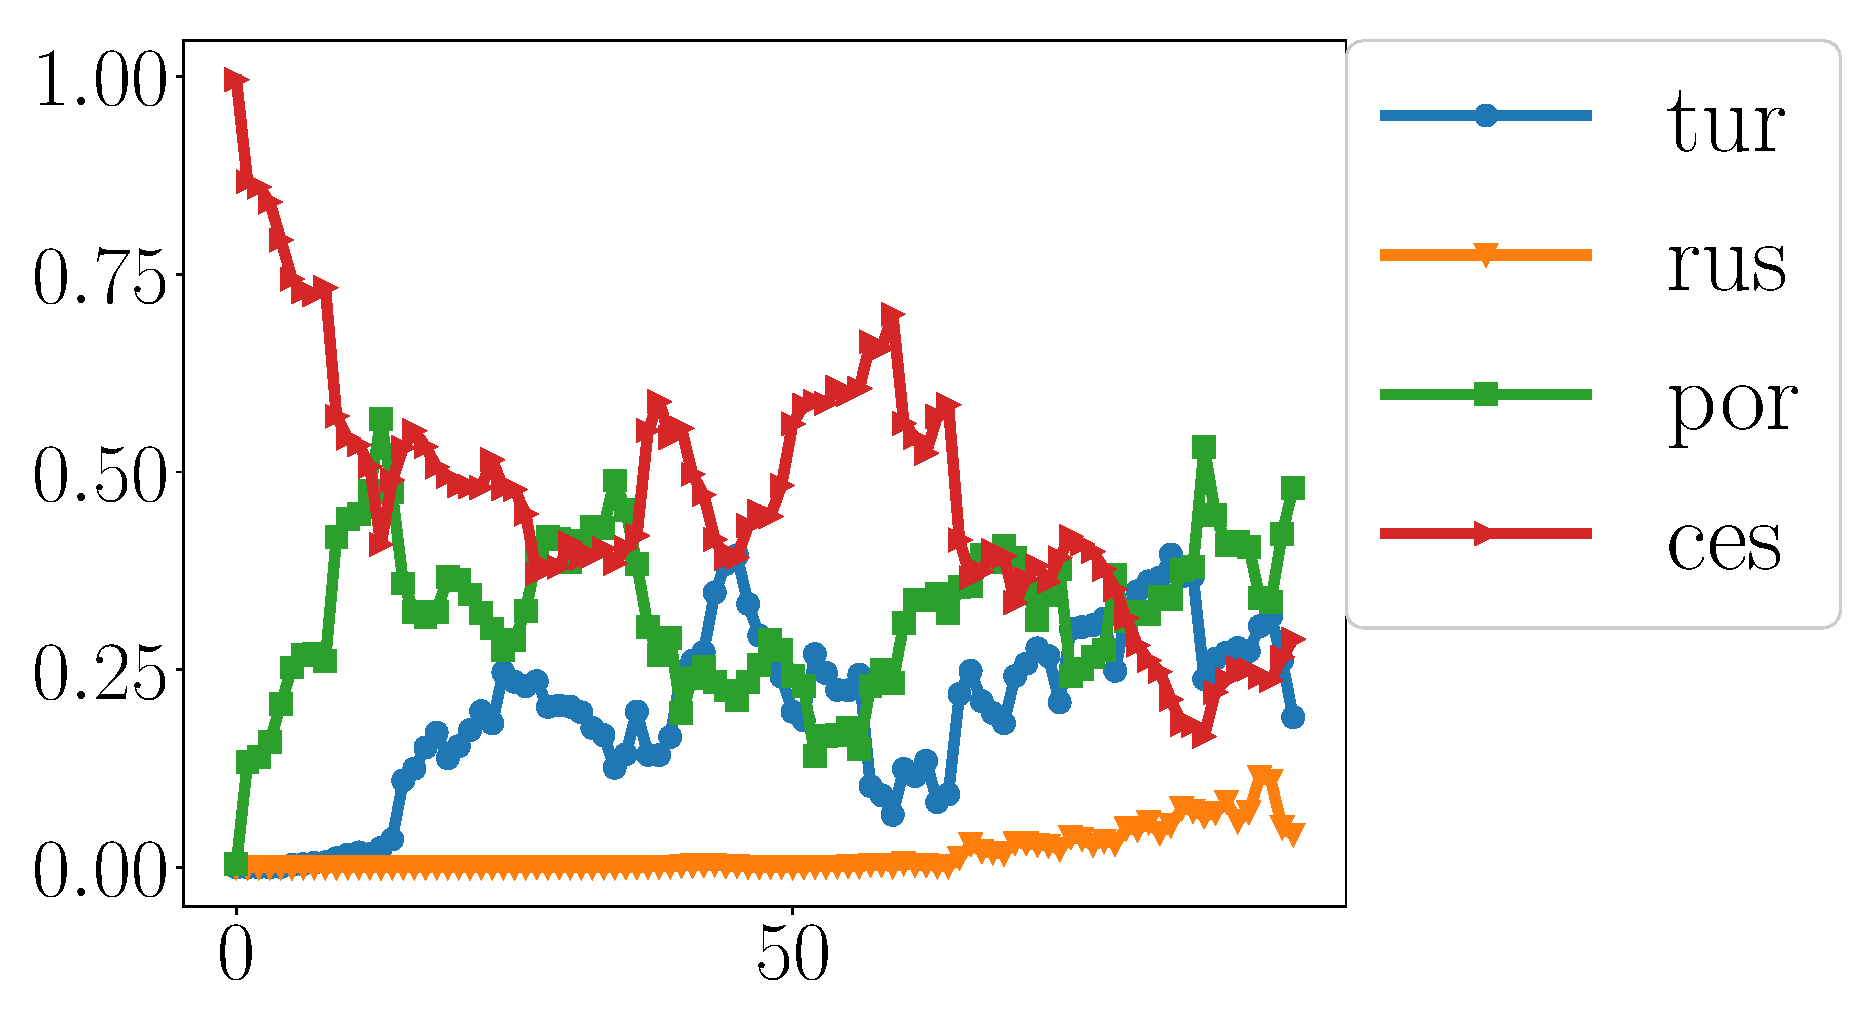
\includegraphics[width=0.29\columnwidth]{figs/slk_hs_probs_plot.eps}
  \captionof{figure}{\label{fig:nmt_distrib_hs}Language usage for TCS$+$DDS vs. training steps. \textit{From left to right}: aze, bel, glg, slk.}
\end{center}

\begin{center}
  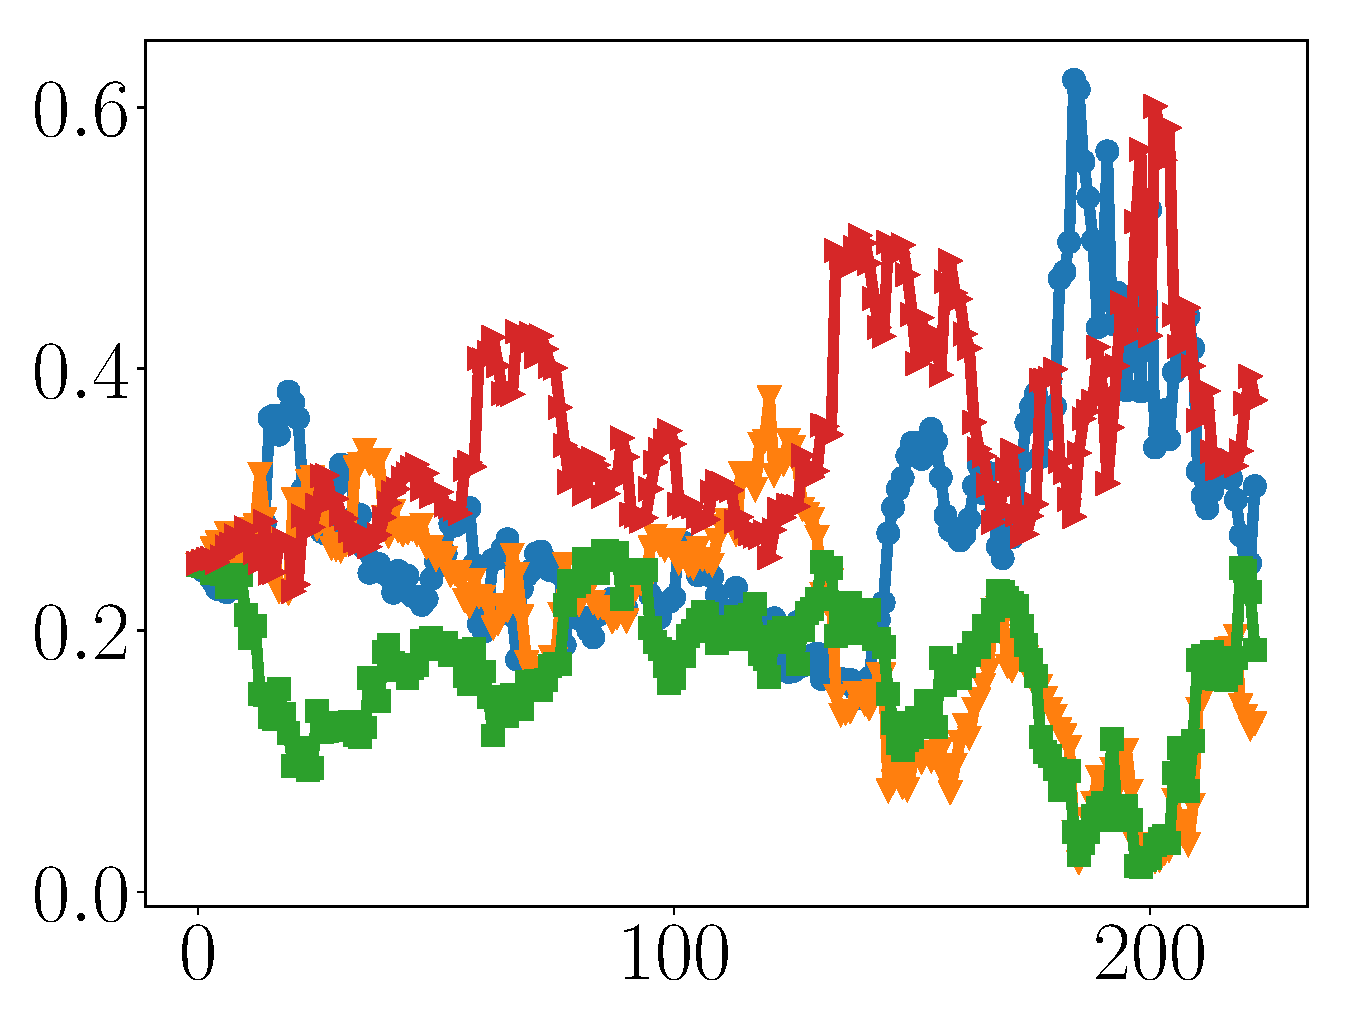
\includegraphics[width=0.22\columnwidth]{figs/aze_uni_probs_plot.eps}
  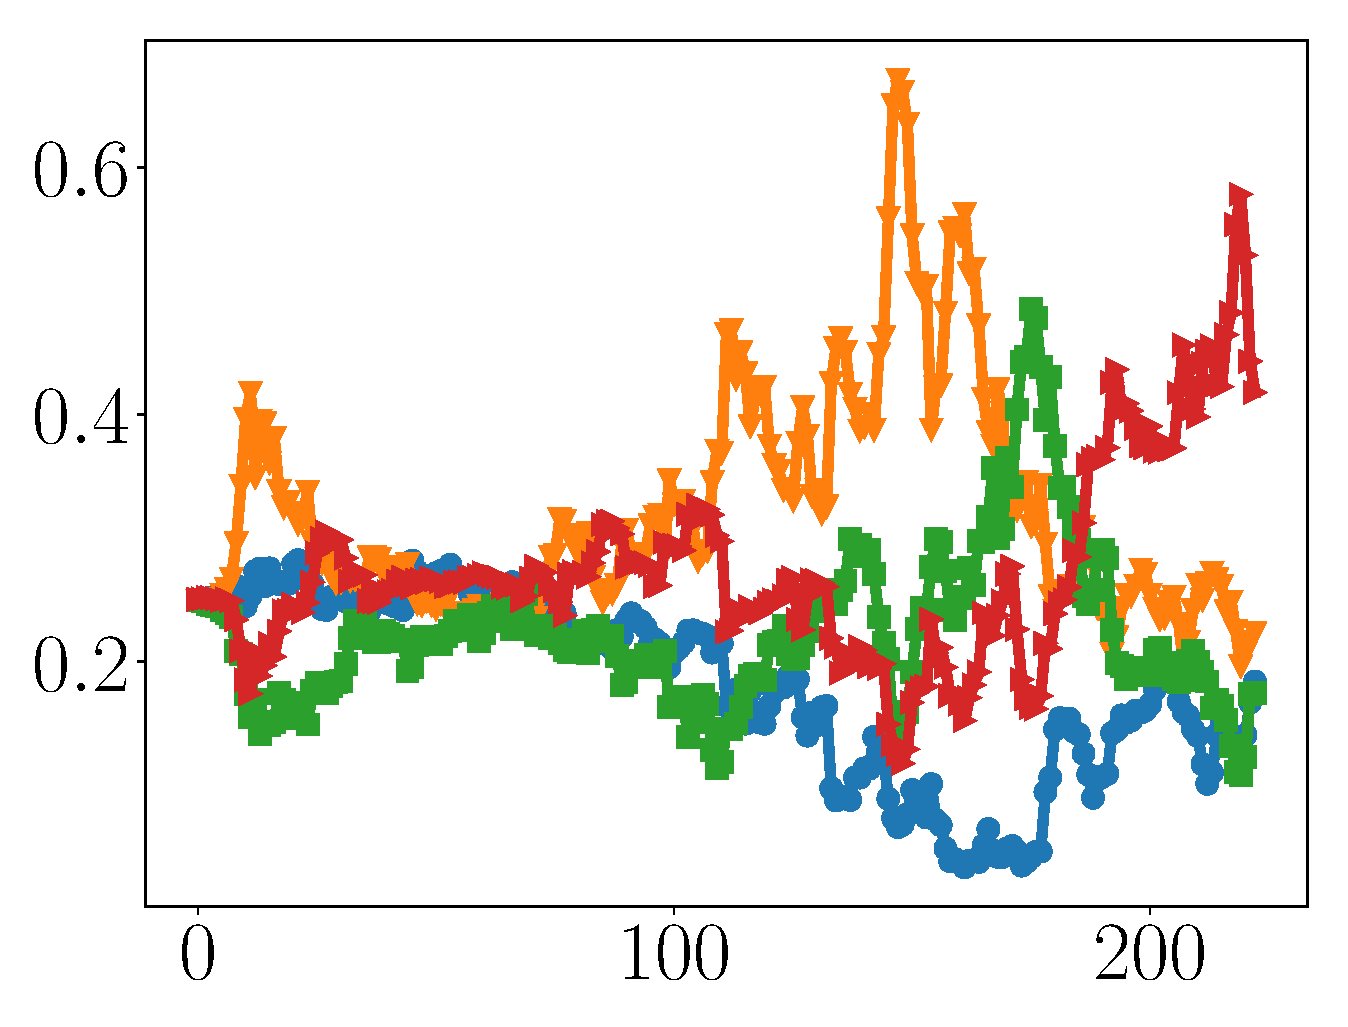
\includegraphics[width=0.22\columnwidth]{figs/bel_uni_probs_plot.eps}
  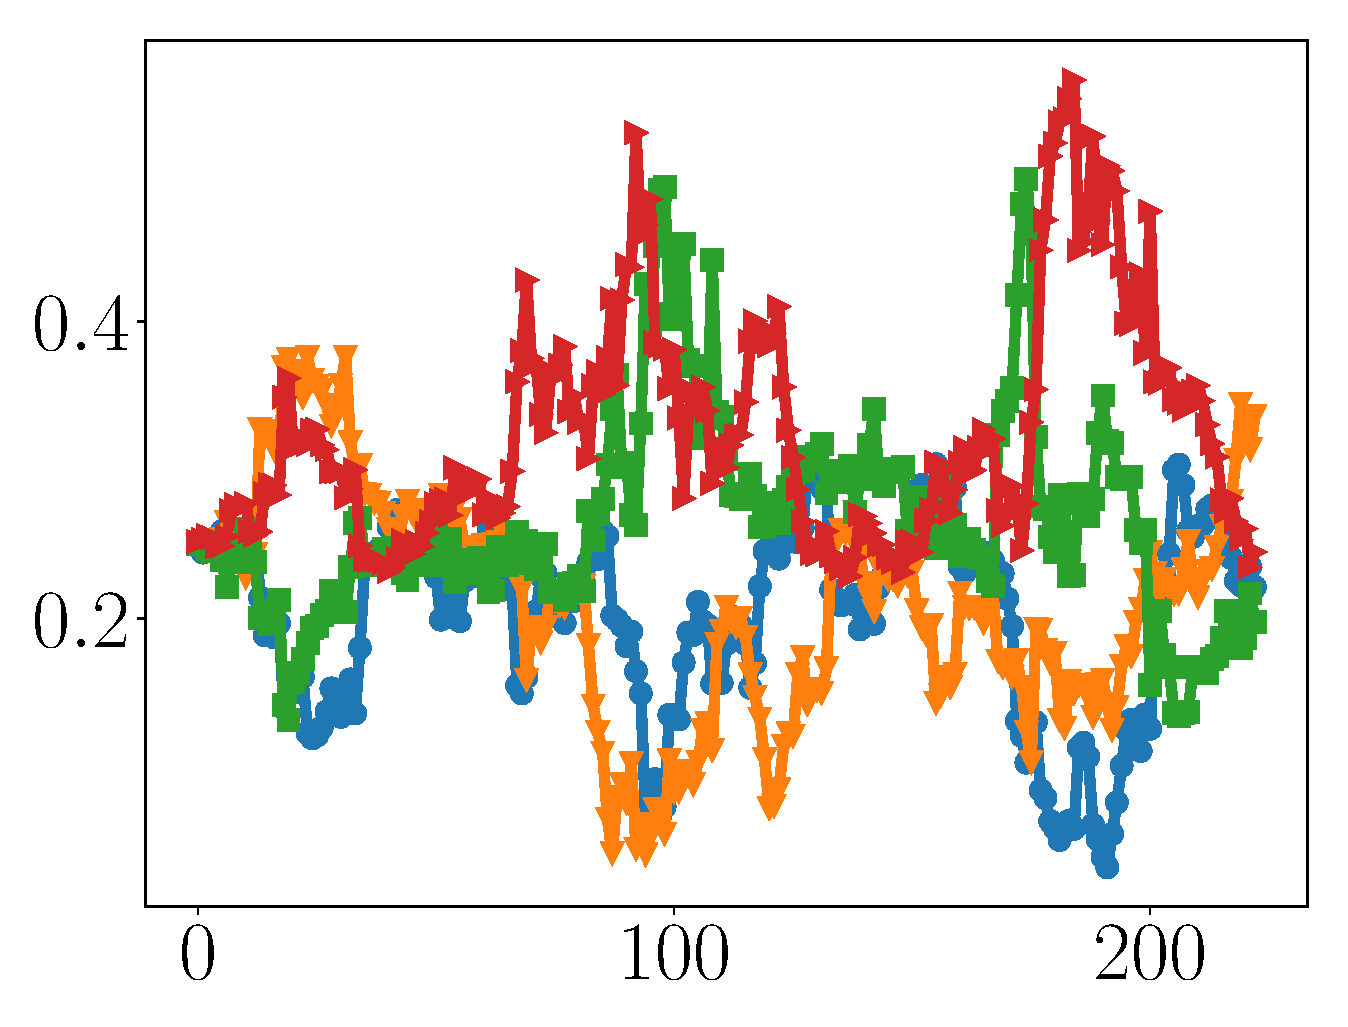
\includegraphics[width=0.22\columnwidth]{figs/glg_uni_probs_plot.eps}
  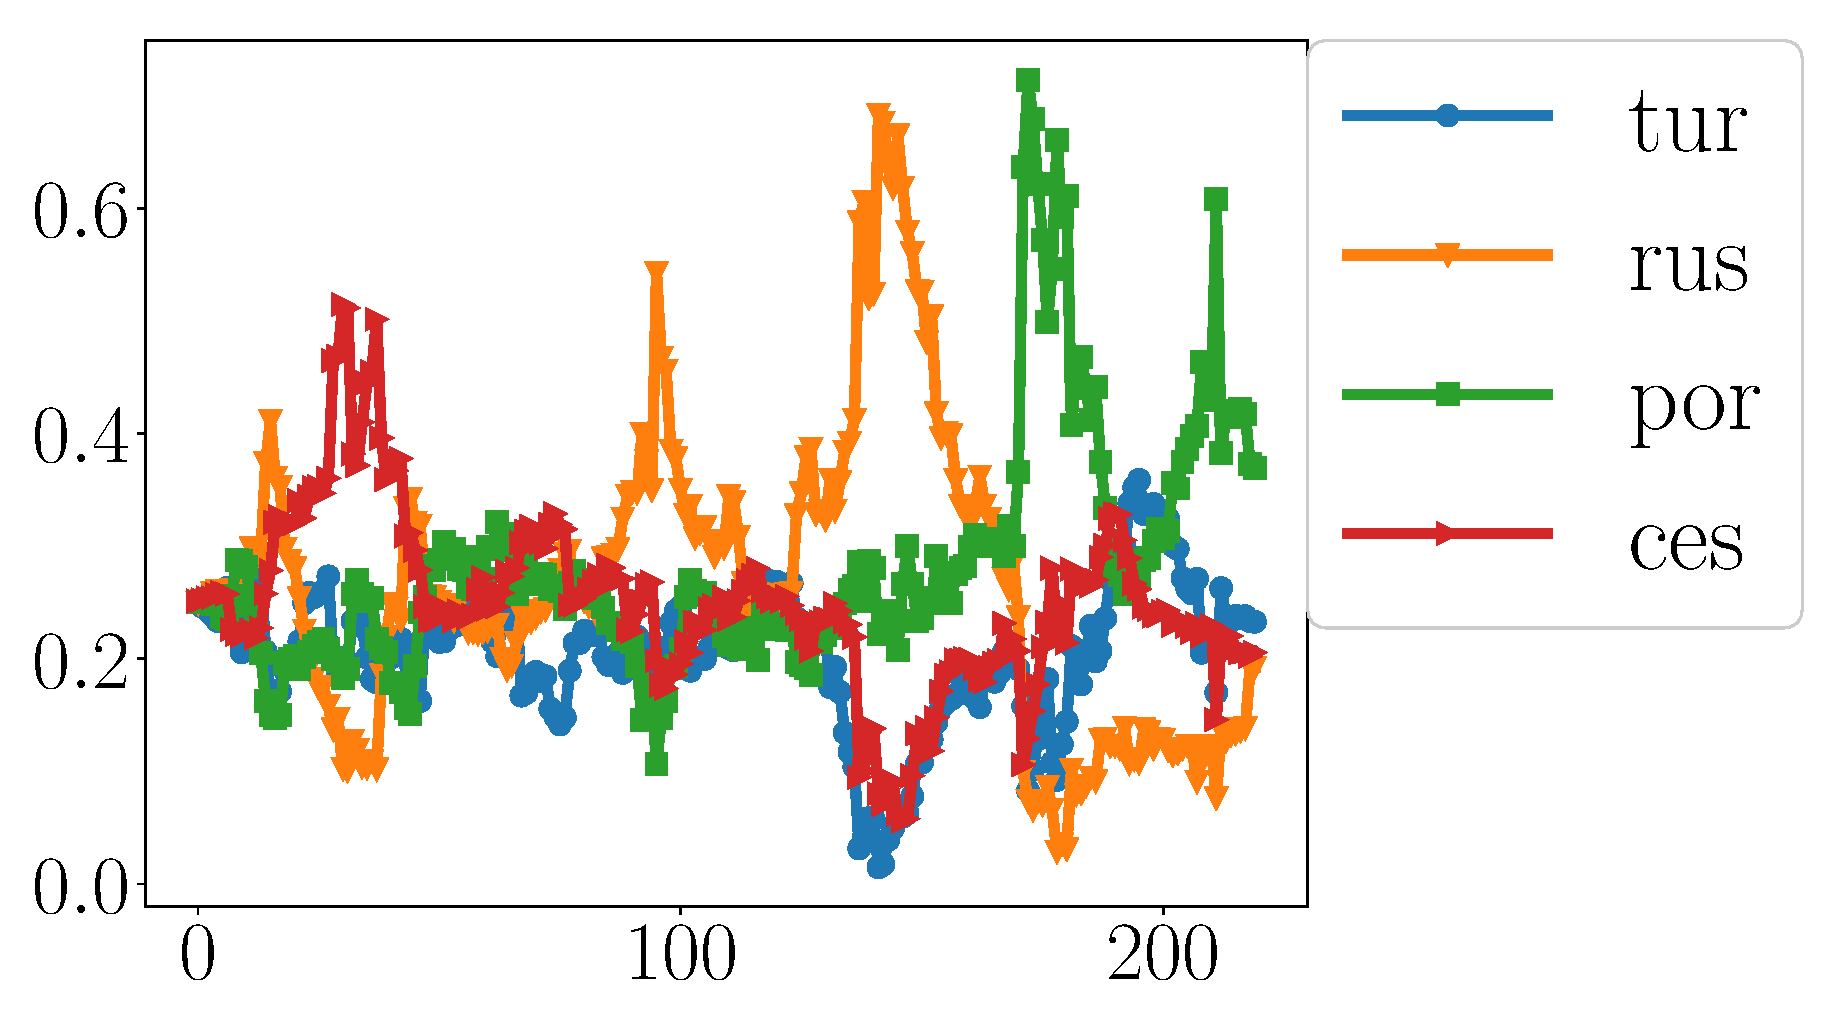
\includegraphics[width=0.29\columnwidth]{figs/slk_uni_probs_plot.eps}
  \captionof{figure}{\label{fig:nmt_distrib_uni}Language usage for Uniform$+$DDS vs. training steps. \textit{From left to right}: aze, bel, glg, slk.}
\end{center}
\paragraph{Learned Language Distribution} To analyze the learned language distribution, we plot the probability distribution of the four HRLs over the course of training. We focus on the four languages because they have the most amount of data and probably affect the model performance more.  Figure \ref{fig:nmt_distrib_hs} shows the change of language distribution for TCS+DDS. Since TCS selects the language with the most number of vocabulary overlap with the LRL, the distribution is initialized to focus on the most related HRL. For all four LRLs, the percentage of their most related HRL start to decrease as training begins. For aze, DDS quickly comes back to using the its most related HRL. However, for bel, DDS continues the trend of using all four languages. This shows that DDS is able to maximize the benefits of the multilingual data by having a more balanced usage of all languages. 
%For gig and slk, DDS learns to mainly use both por and ces, their corresponding HRL.

In Figure \ref{fig:nmt_distrib_uni}, we show a more interesting trend of DDS without heuristic initialization. For both aze and bel, our method learns to focus on their most related HRL after some training updates.
Interestingly, for bel, DDS learns to focus on both rus, the most related HRL for bel, and another language ces. Similarly for slk, DDS also learns to focus on ces, its most related HRL, and rus, although there is little vocabulary overlap between slk and rus. Since DDS does not rely on heuristics, such as vocabulary overlap between languages, it is able to discover better data usage strategies than the already strong heuristic methods such as TCS.
%Similar to the trend in Figure \ref{fig:nmt_distrib_hs}, glg tends to use both por, its most related HRL, and ces. 
